\documentclass{standalone}
\usepackage{tikz}
\usepackage{pgfplots}
\begin{document}
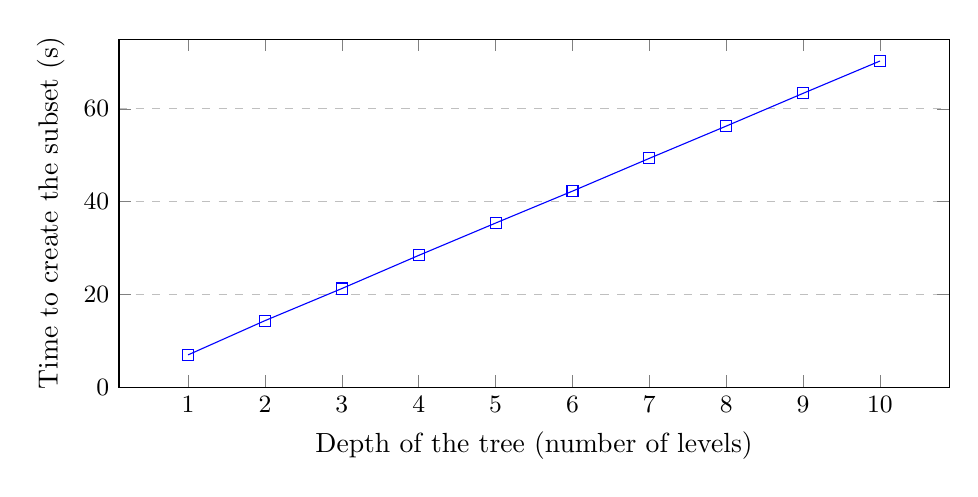
\begin{tikzpicture}
    \begin{axis}[
            title={},
            xlabel={Depth of the tree (number of levels)},
            ylabel={Time to create the subset (s)},
            ymin=0, ymax=75,
            xtick=data,
            height=6cm,
            width=\textwidth,
            legend pos=north west,
            ymajorgrids=true,
            grid style=dashed,
            tick align=inside,
            every tick label/.append style={font=\small}
        ]
        \addplot[
            color=blue,
            mark=square,
        ]
        coordinates {
                (1,6.962351676)
                (2,14.34134667)
                (3,21.2606046)
                (4,28.408648797)
                (5,35.377034333)
                (6,42.260384812)
                (7,49.327177589)
                (8,56.280910516)
                (9,63.340329004)
                (10,70.306947374)
            };
    \end{axis}
\end{tikzpicture}
\end{document}